\chapter{RESULTADOS OBTIDOS}

\section{Desempenho do Algoritmo}

Os resultados obtidos demonstram o desempenho do algoritmo em diferentes configurações de treinamento e teste. Abaixo estão os resultados para cada conjunto de dados de treinamento e teste:

%------------ port

\subsection{Resultados do treinamento com o \textit{dataset Galhardi} (Português) usando o Modelo \textit{BERTimbau Base}}

Os resultados do treinamento com o \textit{dataset Galhardi} em português utilizando o modelo \textit{BERTimbau Base} mostram uma acurácia média variando de 59.35\% a 63.43\%. A acurácia mais alta foi alcançada com 80\% dos dados de treinamento. Apesar de a acurácia média ser menor em comparação com os modelos de inglês e espanhol que serão exibidos em após os resultados em portugês.

\begin{table}[h!]
\centering
\resizebox{\columnwidth}{!}{%
\begin{tabular}{|p{0.25\textwidth}|p{0.1\textwidth}|p{0.1\textwidth}|p{0.4\textwidth}|p{0.1\textwidth}|p{0.1\textwidth}|p{0.1\textwidth}|}
    \hline
    \textbf{Percentual de dados para o treinamento} & \textbf{Qtd. Treino} & \textbf{Qtd. Teste} & \textbf{Pesos [Fator 1, Fator 2, Fator 3]} & \textbf{EQM} & \textbf{EMA} & \textbf{Acurácia média} \\
    \hline
     60\% & 14026 & 9352 & [0.6540, 0.2649, 0.2679] & 0.5211 & 0.5284 & 59.35\% \\
    \hline
     70\% & 16364 & 7014 & [0.6064, 0.2940, 0.2973] & 0.5165 & 0.5262 & 61.46\% \\
    \hline
     80\% & 18702 & 4676 & [0.5772, 0.2574, 0.3362] & 0.5385 & 0.5375 & 63.43\% \\
    \hline
     90\% & 21040 & 2338 & [0.4971, 0.2798, 0.4261] & 0.5950 & 0.5686 & 62.26\% \\
    \hline
\end{tabular}%
}
\caption{Resultados de Regressão para Diferentes Percentuais de Treino com o \textit{dataset Galhardi} (Português) usando o Modelo \textit{BERTimbau Base}}
\label{tab:resultados_regressao_portugues_base}
\end{table}

Nos gŕafico das Figuras \ref{figure:44}, \ref{figure:45}, \ref{figure:46} e \ref{figure:47}  é possível ver uma concetração dos dados na faixa de 40\% até 60\%, com uma queda dessa faixa mais notável na \ref{figure:47}.


\begin{figure}[h!]
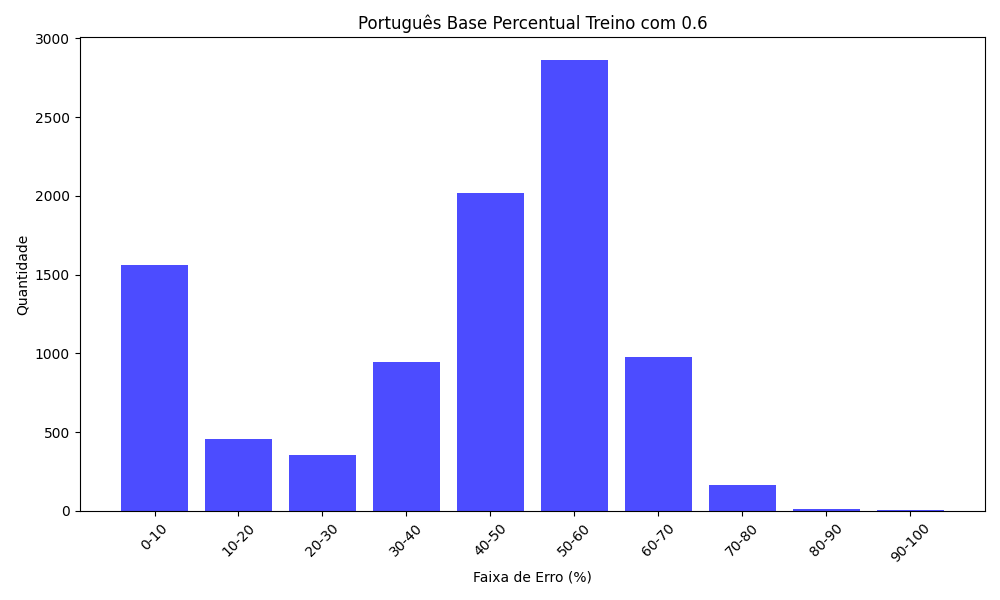
\includegraphics[width=\textwidth]{img/grafsPort/Português Base Percentual Treino com 0.6_quantidade.png}
\caption{Quantidade de respostas por faixas de erro percentual dos testes com 40\% do \textit{dataset Galhardi} (Português) usando o Modelo \textit{BERTimbau Base})}\label{figure:44}
\end{figure}

\begin{figure}[h!]
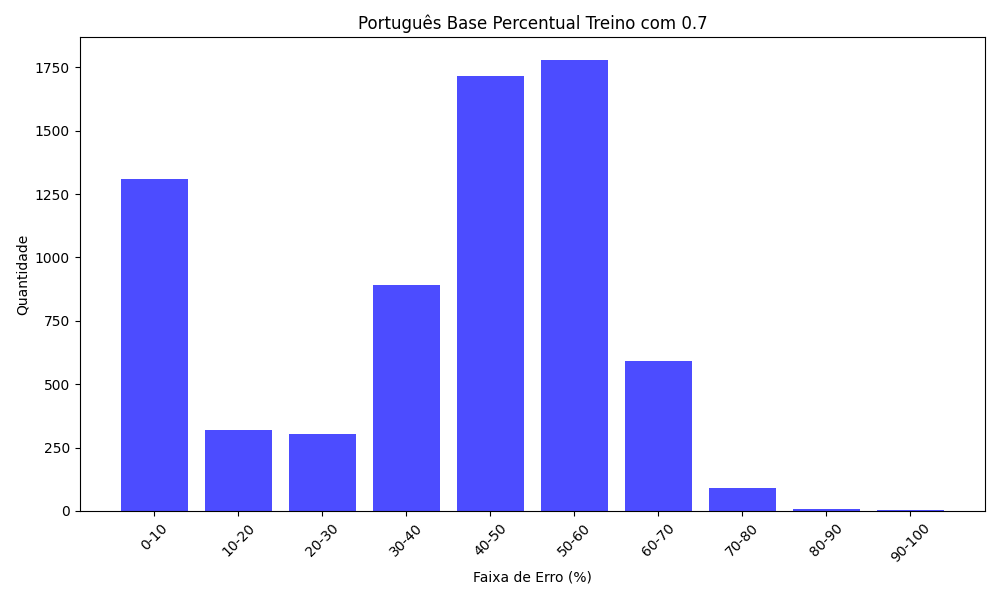
\includegraphics[width=\textwidth]{img/grafsPort/Português Base Percentual Treino com 0.7_quantidade.png}
\caption{Quantidade de respostas por faixas de erro percentual dos testes com 30\% do \textit{dataset Galhardi} (Português) usando o Modelo \textit{BERTimbau Base})}\label{figure:45}
\end{figure}

\begin{figure}[h!]
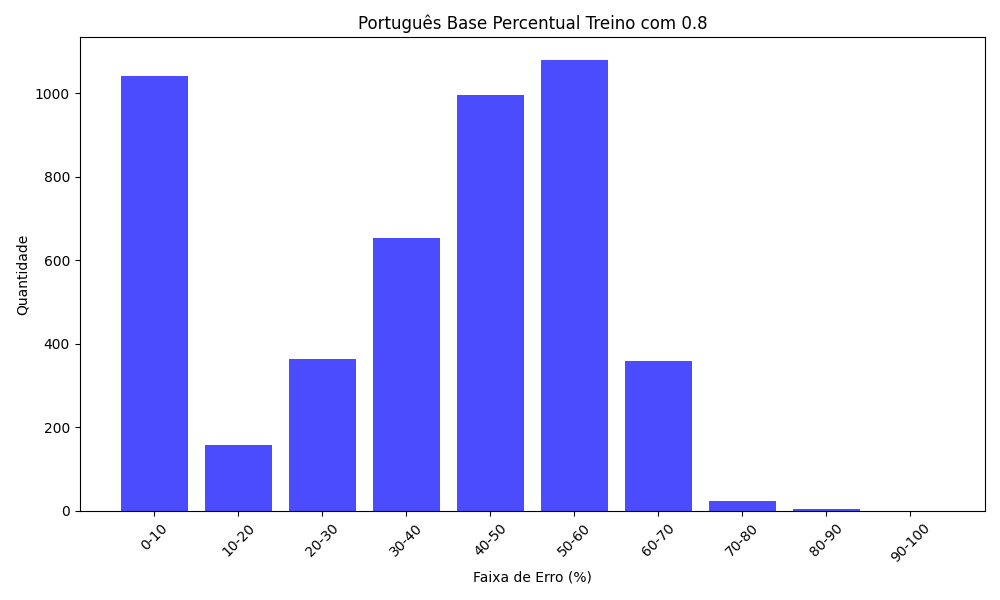
\includegraphics[width=\textwidth]{img/grafsPort/Português Base Percentual Treino com 0.8_quantidade.png}
\caption{Quantidade de respostas por faixas de erro percentual dos testes com 20\% do \textit{dataset Galhardi} (Português) usando o Modelo \textit{BERTimbau Base})}\label{figure:46}
\end{figure}

\begin{figure}[h!]
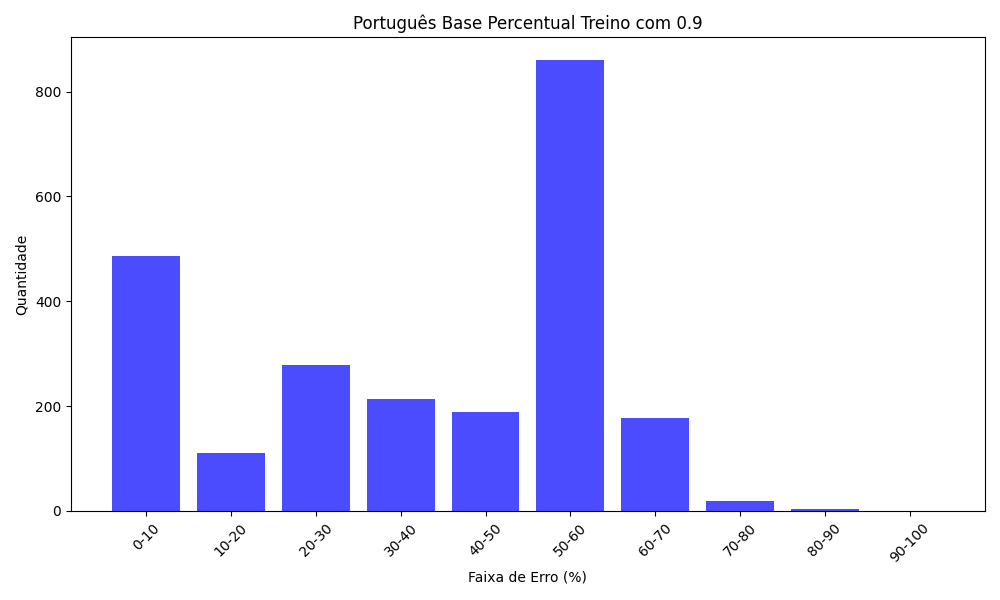
\includegraphics[width=\textwidth]{img/grafsPort/Português Base Percentual Treino com 0.9_quantidade.png}
\caption{Quantidade de respostas por faixas de erro percentual dos testes com 10\% do \textit{dataset Galhardi} (Português) usando o Modelo \textit{BERTimbau Base})}\label{figure:47}
\end{figure}

\FloatBarrier

%--------------------------------------------------

\subsection{Resultados do treinamento com o \textit{dataset Galhardi} (Português) usando o Modelo \textit{BERTimbau Large}}

Os resultados para o \textit{dataset Galhardi} em português utilizando o modelo \textit{BERTimbau Large} indicam uma acurácia média variando entre 55.4\% e 59.83\%. A acurácia mais alta foi obtida com 80\% dos dados de treinamento. Embora a acurácia média seja menor do que a observada com o modelo \textit{BERTimbau Base}, os valores de EQM e EMA sugerem que o modelo \textit{BERTimbau Large} pode precisar de mais ajustes para alcançar um desempenho superior em tarefas de linguagem natural em português, pelo menos quando usado na tarefa de avaliar similaridade semântica.

\begin{table}[h!]
\centering
\resizebox{\columnwidth}{!}{%
\begin{tabular}{|p{0.25\textwidth}|p{0.1\textwidth}|p{0.1\textwidth}|p{0.4\textwidth}|p{0.1\textwidth}|p{0.1\textwidth}|p{0.1\textwidth}|}
    \hline
    \textbf{Percentual de dados para o treinamento} & \textbf{Qtd. Treino} & \textbf{Qtd. Teste} & \textbf{Pesos [Fator 1, Fator 2, Fator 3]} & \textbf{EQM} & \textbf{EMA} & \textbf{Acurácia média} \\
    \hline
    60\% & 14026 & 9352 & [0.7045, 0.2960, 0.5349] & 0.5230 & 0.5318 & 55.4\% \\
    \hline
    70\% & 16364 & 7014 & [0.6538, 0.3434, 0.5882] & 0.5201 & 0.5317 & 58.14\% \\
    \hline
    80\% & 18702 & 4676 & [0.6335, 0.3061, 0.6643] & 0.5438 & 0.5443 & 59.83\% \\
    \hline
    90\% & 21040 & 2338 & [0.5673, 0.3484, 0.8416] & 0.6037 & 0.5765 & 57.91\% \\
    \hline
\end{tabular}%
}
\caption{Resultados de Regressão para Diferentes Percentuais de Treino com o \textit{dataset Galhardi} (Português) usando o Modelo \textit{BERTimbau Large}}
\label{tab:resultados_regressao_portugues_large}
\end{table}

Nos gŕafico das Figura \ref{figure:34} é possível ver uma concetração dos dados na faixa de 50\% até 70\%, embora na Figura \ref{figure:37} o erro pareça menor, ainda é possível notar que esse faixa possui mais concentração que as outras.

\begin{figure}[h!]
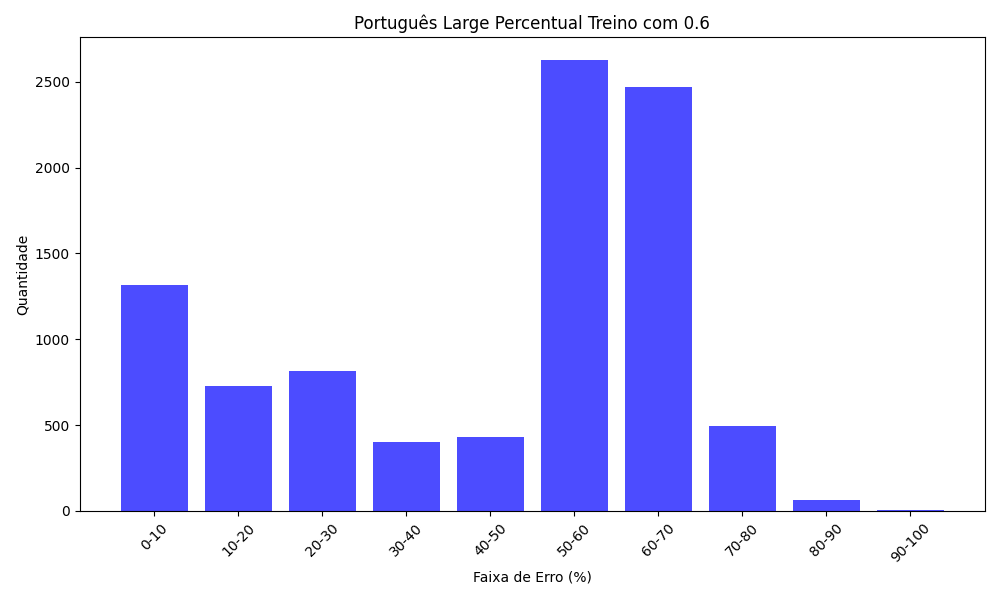
\includegraphics[width=\textwidth]{img/grafsPort/Português Large Percentual Treino com 0.6_quantidade.png}
\caption{Quantidade de respostas por faixas de erro percentual dos testes com 40\% do \textit{dataset Galhardi} (Português) usando o Modelo \textit{BERTimbau Large})}\label{figure:34}
\end{figure}

\begin{figure}[h!]
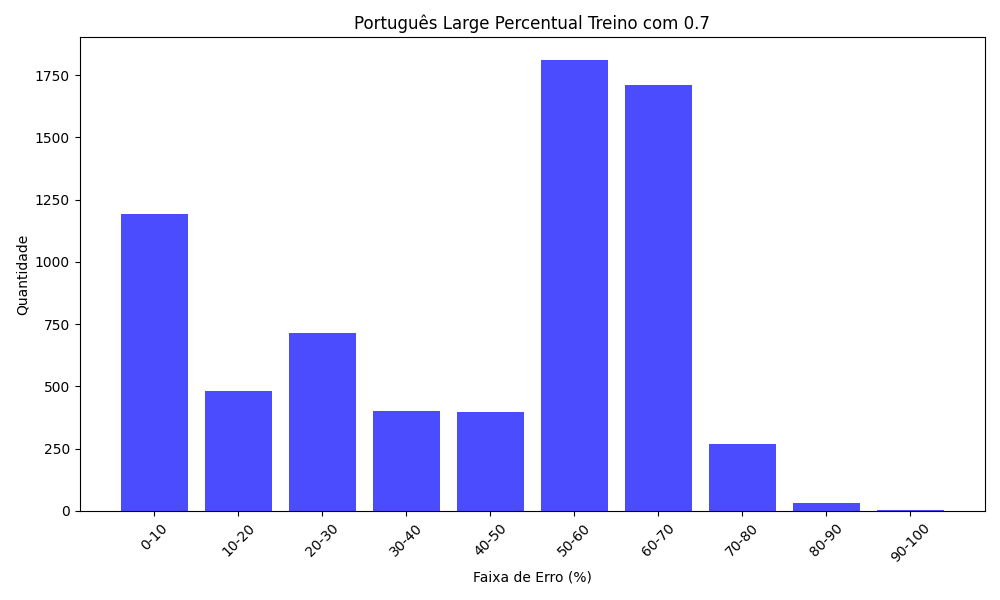
\includegraphics[width=\textwidth]{img/grafsPort/Português Large Percentual Treino com 0.7_quantidade.png}
\caption{Quantidade de respostas por faixas de erro percentual dos testes com 30\% do \textit{dataset Galhardi} (Português) usando o Modelo \textit{BERTimbau Large})}\label{figure:35}
\end{figure}

\begin{figure}[h!]
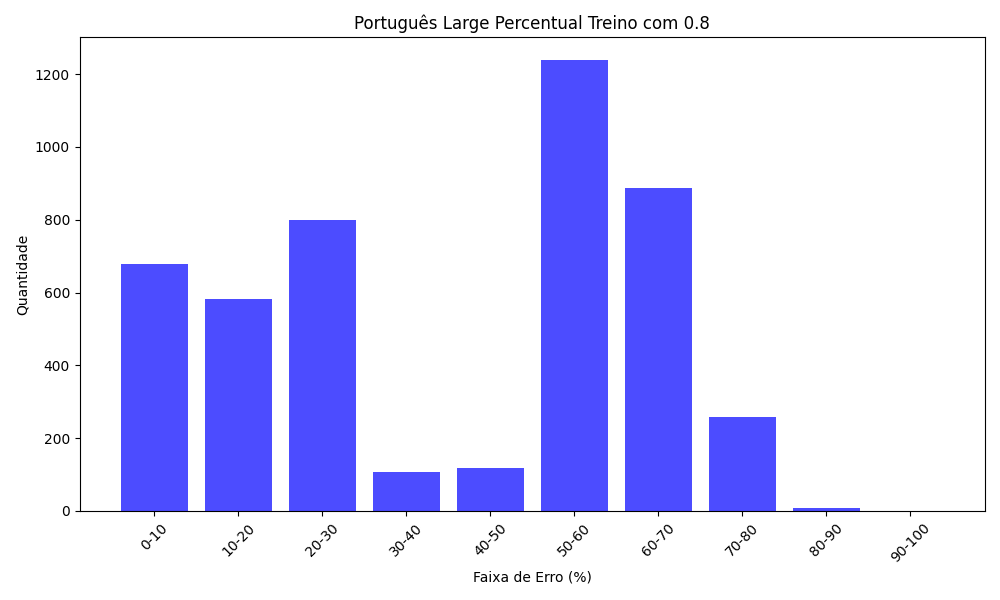
\includegraphics[width=\textwidth]{img/grafsPort/Português Large Percentual Treino com 0.8_quantidade.png}
\caption{Quantidade de respostas por faixas de erro percentual dos testes com 20\% do \textit{dataset Galhardi} (Português) usando o Modelo \textit{BERTimbau Large})}\label{figure:36}
\end{figure}

\begin{figure}[h!]
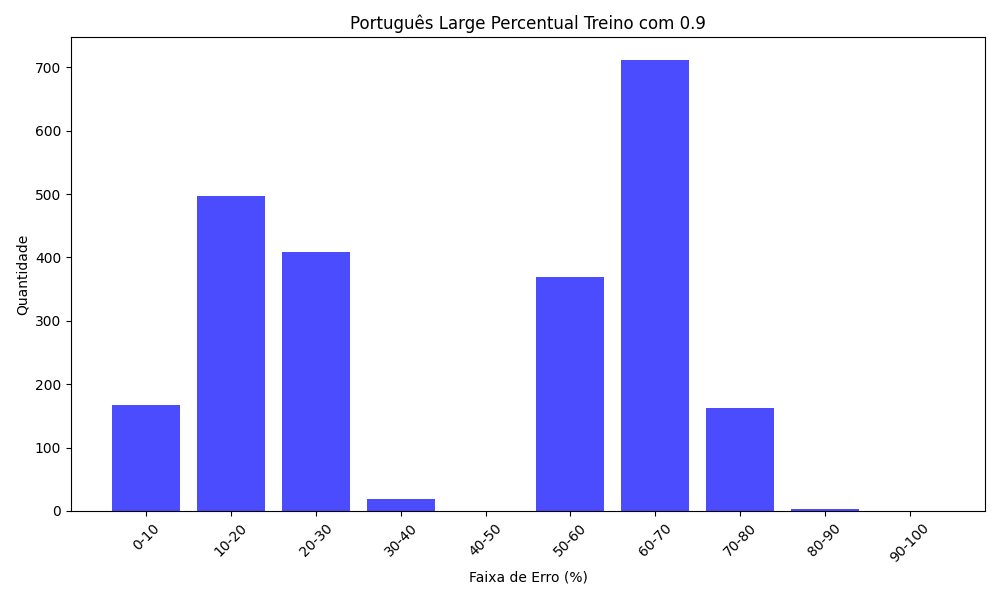
\includegraphics[width=\textwidth]{img/grafsPort/Português Large Percentual Treino com 0.9_quantidade.png}
\caption{Quantidade de respostas por faixas de erro percentual dos testes com 10\% do \textit{dataset Galhardi} (Português) usando o Modelo \textit{BERTimbau Large})}\label{figure:37}
\end{figure}

\FloatBarrier

%------------ esp

\subsection{Resultados do treinamento com o \textit{dataset Mardini} (Espanhol) usando o Modelo \textit{BETO Base}}

Os resultados para o \textit{dataset Mardini} em espanhol utilizando o modelo \textit{BETO Base} demonstram uma acurácia média variando entre 65.12\% e 71.7\%. A acurácia mais alta foi alcançada com 90\% dos dados de treinamento. Os valores de EQM e EMA são relativamente estáveis, com uma leve melhoria à medida que a quantidade de dados de treinamento aumenta. Estes resultados indicam que o modelo \textit{BETO Base} é eficaz para tarefas em espanhol, embora haja espaço para melhorias no uso de outra versão do modelo, como veremos na comparação a versão \textit{Large}.

\begin{table}[h!]
\centering
\resizebox{\columnwidth}{!}{%
\begin{tabular}{|p{0.25\textwidth}|p{0.1\textwidth}|p{0.1\textwidth}|p{0.4\textwidth}|p{0.1\textwidth}|p{0.1\textwidth}|p{0.1\textwidth}|}
    \hline
    \textbf{Percentual de dados para o treinamento} & \textbf{Qtd. Treino} & \textbf{Qtd. Teste} & \textbf{Pesos [Fator 1, Fator 2, Fator 3]} & \textbf{EQM} & \textbf{EMA} & \textbf{Acurácia média} \\
    \hline
     60\% & 2263 & 1509 & [0.0838, 0.0349, 0.4526] & 0.8955 & 0.7457 & 65.12\% \\
    \hline
     70\% & 2640 & 1132 & [0.1119, 0.0387, 0.4619] & 0.9010 & 0.7536 & 66.58\% \\
    \hline
     80\% & 3017 & 755 & [0.1077, 0.0453, 0.4709] & 0.8702 & 0.7390 & 66.28\% \\
    \hline
     90\% & 3394 & 378 & [0.1034, 0.0486, 0.4504] & 0.8822 & 0.7449 & 71.7\% \\
    \hline
\end{tabular}%
}
\caption{Resultados de Regressão para Diferentes Percentuais de Treino com o \textit{dataset Mardini} (Espanhol) usando o Modelo \textit{BETO Base}}
\label{tab:resultados_regressao_espanhol_base}
\end{table}

Nos gŕafico das Figuras \ref{figure:4} é possível ver uma quantidade grande de erros distribuídos em varias faixas, ao passo que na Figura \ref{figure:7} esses erros diminuíram, e a faixa mais concetrada é a de entre 20\% e 30\% de divergência nas avaliações do algoritmo comparadas com as avaliações dos professores.

\begin{figure}[h!]
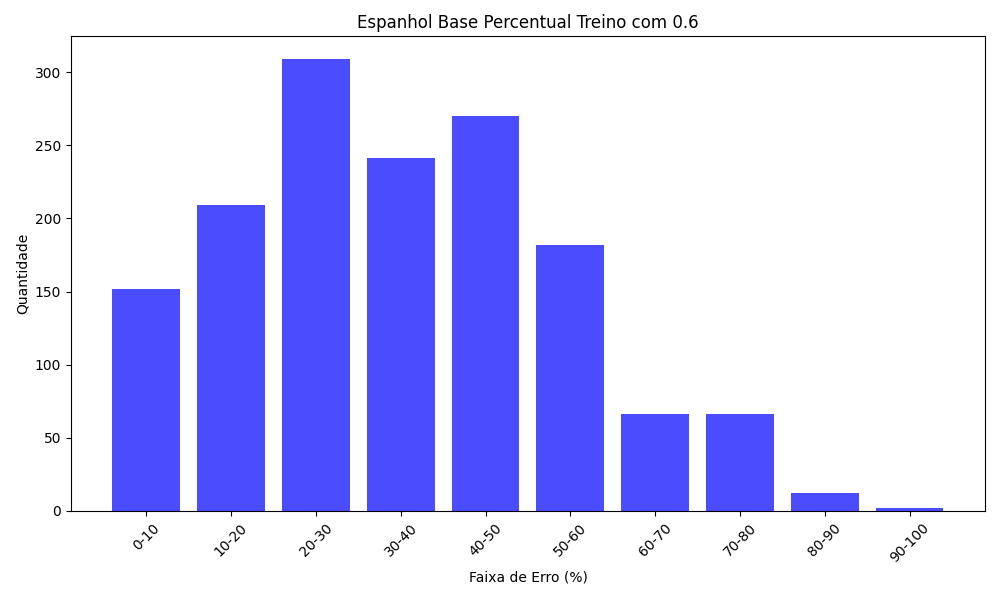
\includegraphics[width=\textwidth]{img/grafsEsp/Espanhol Base Percentual Treino com 0.6_quantidade.png}
\caption{Quantidade de respostas por faixas de erro percentual dos testes com 40\% do \textit{dataset Mardini} (Espanhol) usando o Modelo \textit{BETO Base}}\label{figure:4}
\end{figure}

\begin{figure}[h!]
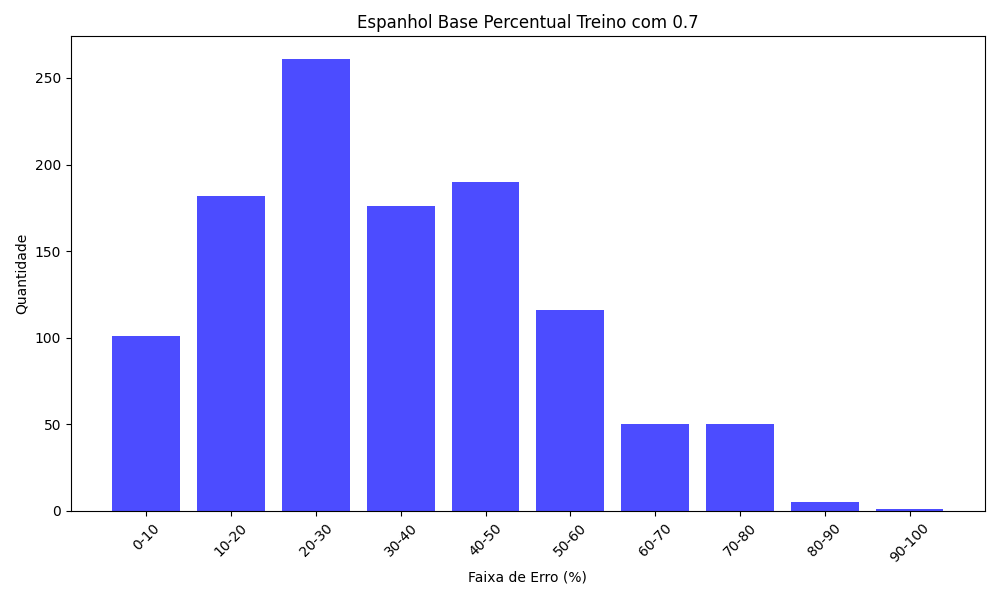
\includegraphics[width=\textwidth]{img/grafsEsp/Espanhol Base Percentual Treino com 0.7_quantidade.png}
\caption{Quantidade de respostas por faixas de erro percentual dos testes com 30\% do \textit{dataset Mardini} (Espanhol) usando o Modelo \textit{BETO Base}}\label{figure:5}
\end{figure}

\begin{figure}[h!]
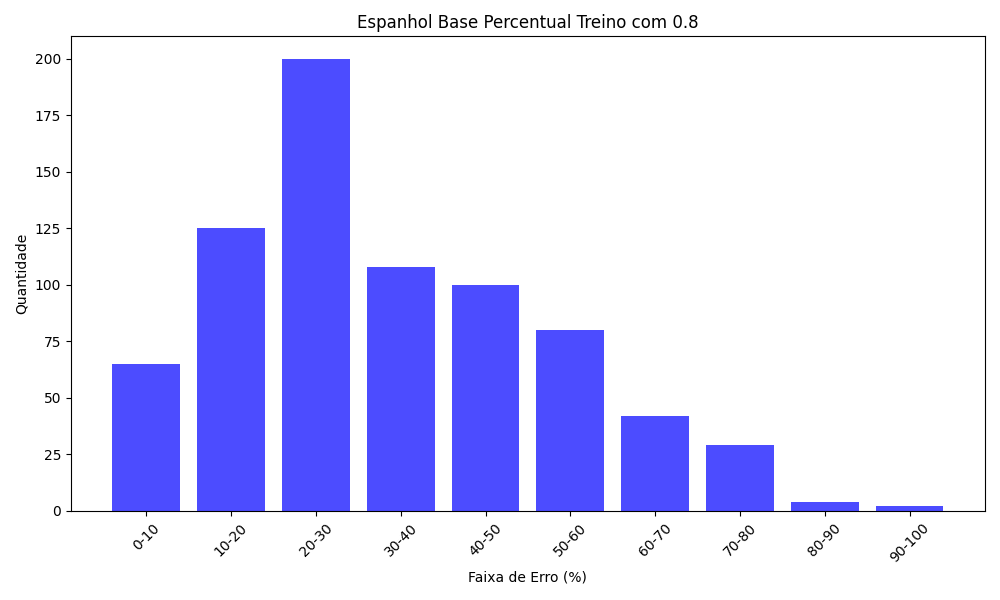
\includegraphics[width=\textwidth]{img/grafsEsp/Espanhol Base Percentual Treino com 0.8_quantidade.png}
\caption{Quantidade de respostas por faixas de erro percentual dos testes com 20\% do \textit{dataset Mardini} (Espanhol) usando o Modelo \textit{BETO Base}}\label{figure:6}
\end{figure}

\begin{figure}[h!]
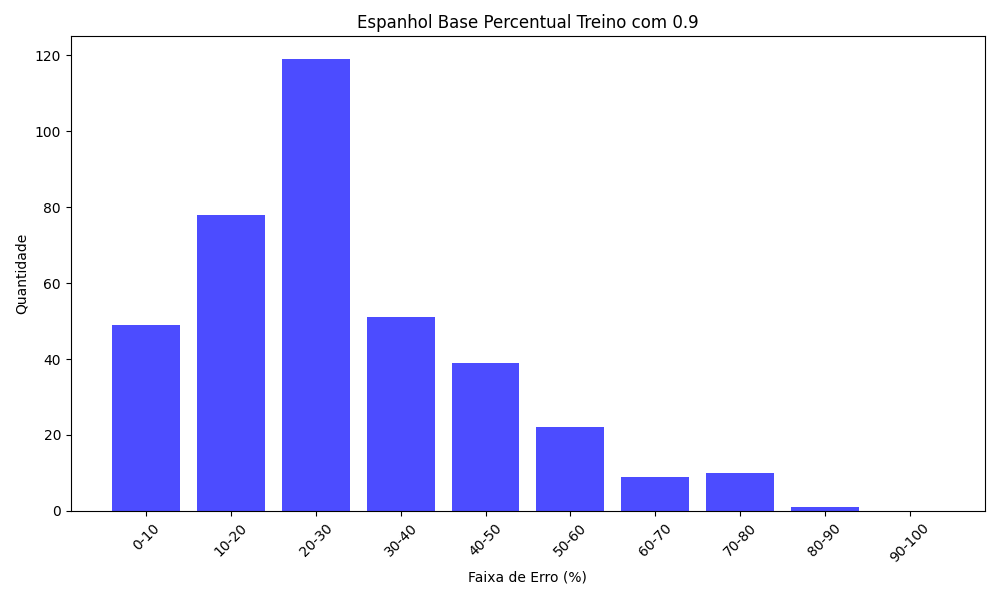
\includegraphics[width=\textwidth]{img/grafsEsp/Espanhol Base Percentual Treino com 0.9_quantidade.png}
\caption{Quantidade de respostas por faixas de erro percentual dos testes com 10\% do \textit{dataset Mardini} (Espanhol) usando o Modelo \textit{BETO Base}}\label{figure:7}
\end{figure}

\FloatBarrier

%-------------------------------------------

\subsection{Resultados do treinamento com o \textit{dataset Mardini} (Espanhol) usando o Modelo \textit{BETO Large}}

Para o \textit{dataset Mardini} em espanhol utilizando o modelo \textit{BETO Large}, os resultados mostram uma acurácia média superior, variando de 78.14\% a 83.58\%. A acurácia mais alta foi obtida com 90\% dos dados de treinamento. Os valores de EQM e EMA são ligeiramente melhores comparados ao modelo \textit{BETO Base}, confirmando que o \textit{BETO Large} oferece um desempenho aprimorado em tarefas de processamento de linguagem natural em espanhol.

\begin{table}[h!]
\centering
\resizebox{\columnwidth}{!}{%
\begin{tabular}{|p{0.25\textwidth}|p{0.1\textwidth}|p{0.1\textwidth}|p{0.4\textwidth}|p{0.1\textwidth}|p{0.1\textwidth}|p{0.1\textwidth}|}
    \hline
    \textbf{Percentual de dados para o treinamento} & \textbf{Qtd. Treino} & \textbf{Qtd. Teste} & \textbf{Pesos [Fator 1, Fator 2, Fator 3]} & \textbf{EQM} & \textbf{EMA} & \textbf{Acurácia média} \\
    \hline
    60\% & 2263 & 1509 & [0.1412, 0.0081, 0.1289] & 0.9622 & 0.7773 & 78.14\% \\
    \hline
    70\% & 2640 & 1132 & [0.1634, 0.0049, 0.1366] & 0.9703 & 0.7835 & 78.74\% \\
    \hline
    80\% & 3017 & 755 & [0.1638, 0.0010, 0.1300] & 0.9450 & 0.7754 & 79.18\% \\
    \hline
    90\% & 3394 & 378 & [0.1509, 0.0085, 0.1439] & 0.9441 & 0.7783 & 83.58\% \\
    \hline
\end{tabular}%
}
\caption{Resultados de Regressão para Diferentes Percentuais de Treino com o \textit{dataset Mardini} (Espanhol) usando o Modelo \textit{BETO Large}}
\label{tab:resultados_regressao_espanhol_large}
\end{table}

Nos gŕafico das Figuras \ref{figure:8}, \ref{figure:9}, \ref{figure:10} e \ref{figure:11} é possível ver que a maiora das avaliações se mantém na faixa de acurácia acima de 70\%, com uma mudança na distribuiçao comparando com o modelo \textit{Base}.

\begin{figure}[h!]
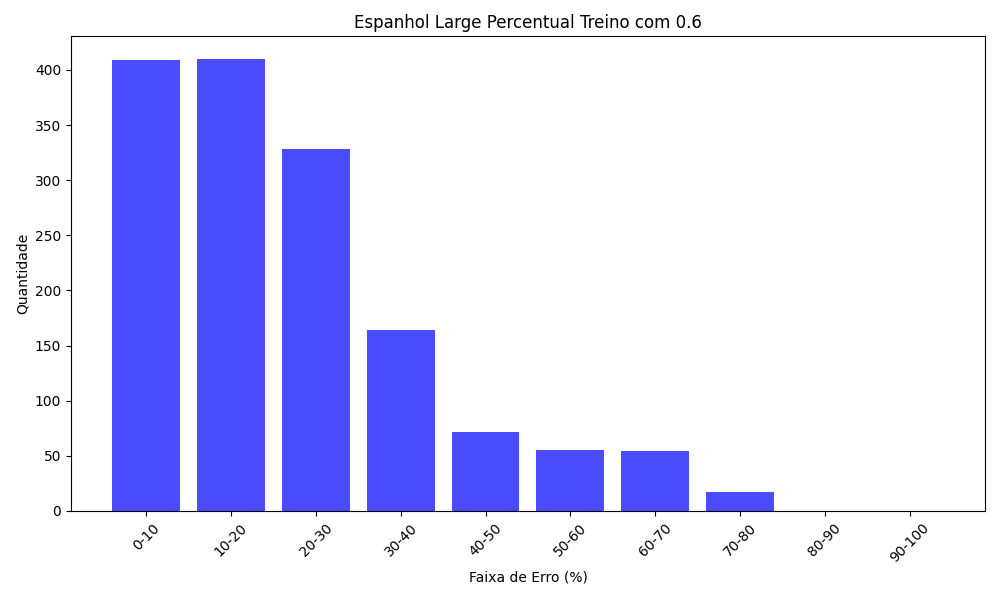
\includegraphics[width=\textwidth]{img/grafsEsp/Espanhol Large Percentual Treino com 0.6_quantidade.png}
\caption{Quantidade de respostas por faixas de erro percentual dos testes com 40\% do \textit{dataset Mardini} (Espanhol) usando o Modelo \textit{BETO Large}}\label{figure:8}
\end{figure}

\begin{figure}[h!]
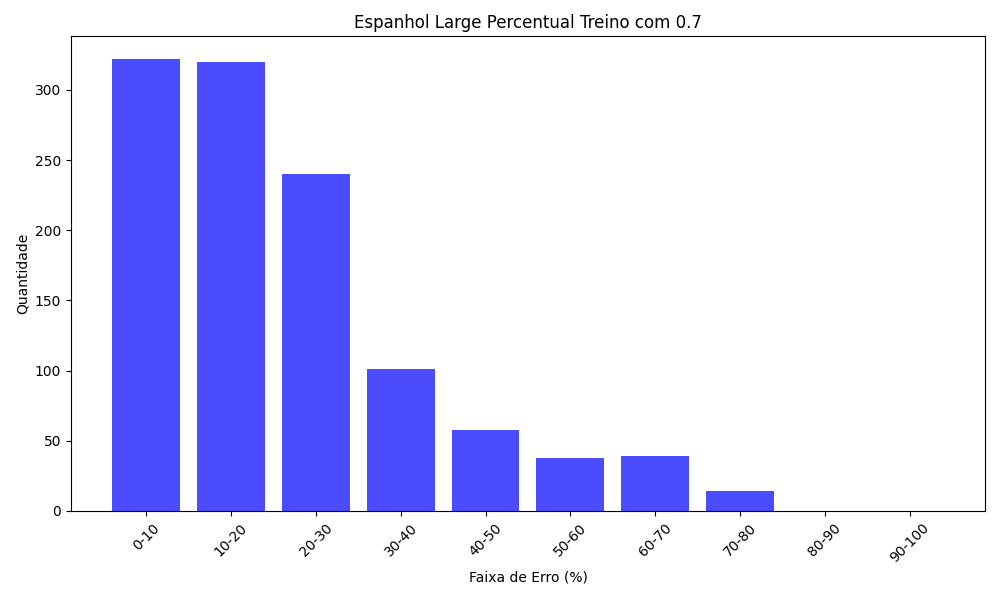
\includegraphics[width=\textwidth]{img/grafsEsp/Espanhol Large Percentual Treino com 0.7_quantidade.png}
\caption{Quantidade de respostas por faixas de erro percentual dos testes com 30\% do \textit{dataset Mardini} (Espanhol) usando o Modelo \textit{BETO Large}}\label{figure:9}
\end{figure}

\begin{figure}[h!]
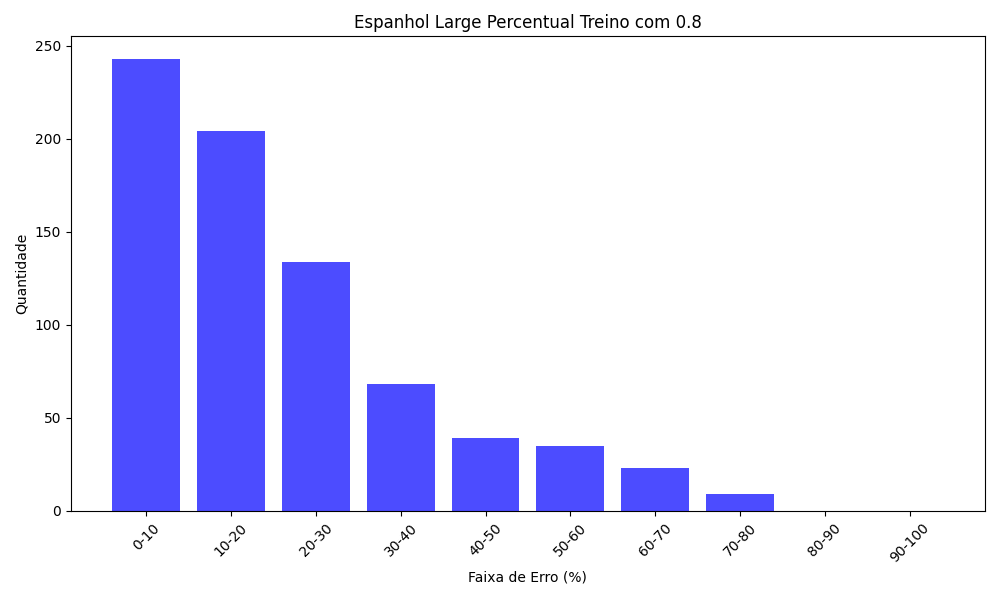
\includegraphics[width=\textwidth]{img/grafsEsp/Espanhol Large Percentual Treino com 0.8_quantidade.png}
\caption{Quantidade de respostas por faixas de erro percentual dos testes com 20\% do \textit{dataset Mardini} (Espanhol) usando o Modelo \textit{BETO Large}}\label{figure:10}
\end{figure}

\begin{figure}[h!]
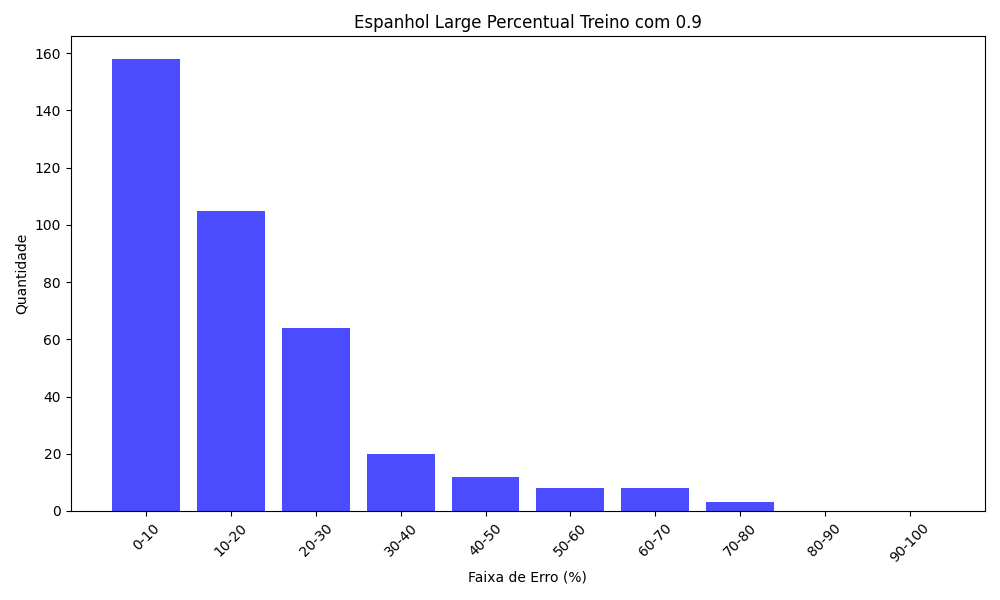
\includegraphics[width=\textwidth]{img/grafsEsp/Espanhol Large Percentual Treino com 0.9_quantidade.png}
\caption{Quantidade de respostas por faixas de erro percentual dos testes com 10\% do \textit{dataset Mardini} (Espanhol) usando o Modelo \textit{BETO Large}}\label{figure:11}
\end{figure}

\FloatBarrier

%-------------------------------------------

% \subsection{Resultados do treinamento com o \textit{dataset} Espanhol usando o Modelo ROBERTA (Quantidade de dados: 3772)}

% \begin{table}[h!]
% \centering
% \resizebox{\columnwidth}{!}{%
% \begin{tabular}{|p{0.25\textwidth}|p{0.1\textwidth}|p{0.1\textwidth}|p{0.4\textwidth}|p{0.1\textwidth}|p{0.1\textwidth}|p{0.1\textwidth}|}
%     \hline
%     \textbf{Percentual de dados para o treinamento} & \textbf{Qtd. Treino} & \textbf{Qtd. Teste} & \textbf{Pesos [Fator 1, Fator 2, Fator 3]} & \textbf{EQM} & \textbf{EMA} & \textbf{Acurácia média} \\
%     \hline
%     60\% & 2263 & 1509 & [0.1782, 0.0090, 0.1067] & 0.9754 & 0.7780 & 74.5\% \\
%     \hline
%     70\% & 2640 & 1132 & [0.2071, 0.0208, 0.1106] & 0.9852 & 0.7867 & 74.98\% \\
%     \hline
%     80\% & 3017 & 755 & [0.2039, 0.0283, 0.1627] & 0.9508 & 0.7734 & 72.66\% \\
%     \hline
%     90\% & 3394 & 378 & [0.1949, 0.0387, 0.1686] & 0.9526 & 0.7774 & 76.27\% \\
%     \hline
% \end{tabular}%
% }
% \caption{Resultados de Regressão para Diferentes Percentuais de Treino com o \textit{dataset} Espanhol usando o modelo ROBERTA}
% \label{tab:resultados_regressao_roberta_espanhol}
% \end{table}

% \begin{figure}[h!]
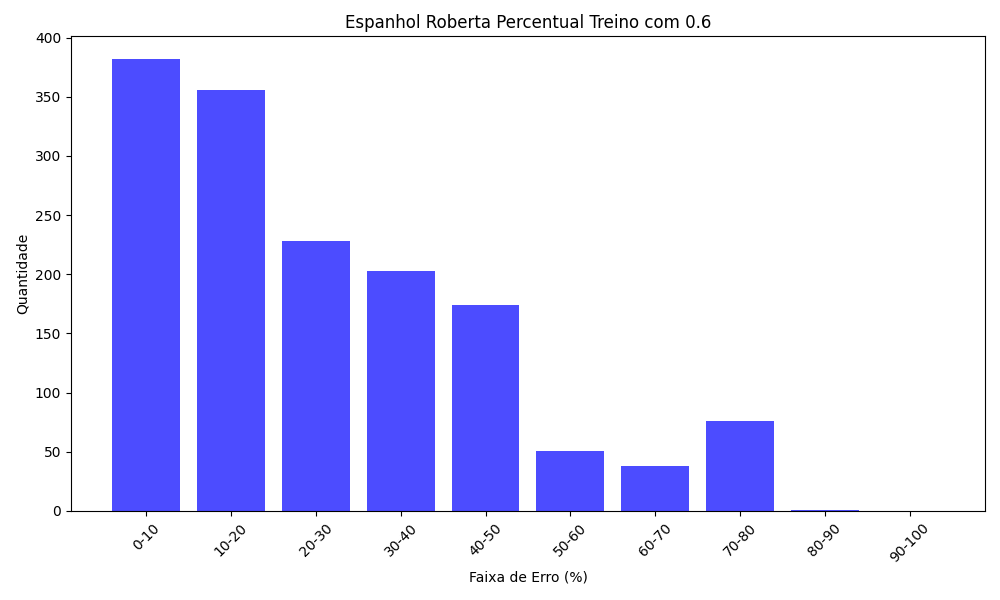
\includegraphics[width=\textwidth]{img/grafsEsp/Espanhol Roberta Percentual Treino com 0.6_quantidade.png}
\caption{Quantidade de respostas por faixas de erro percentual dos testes com 40\% do \textit{dataset} (Modelo Espanhol \textit{ROBERTA})}\label{figure:12}
\end{figure}

\begin{figure}[h!]
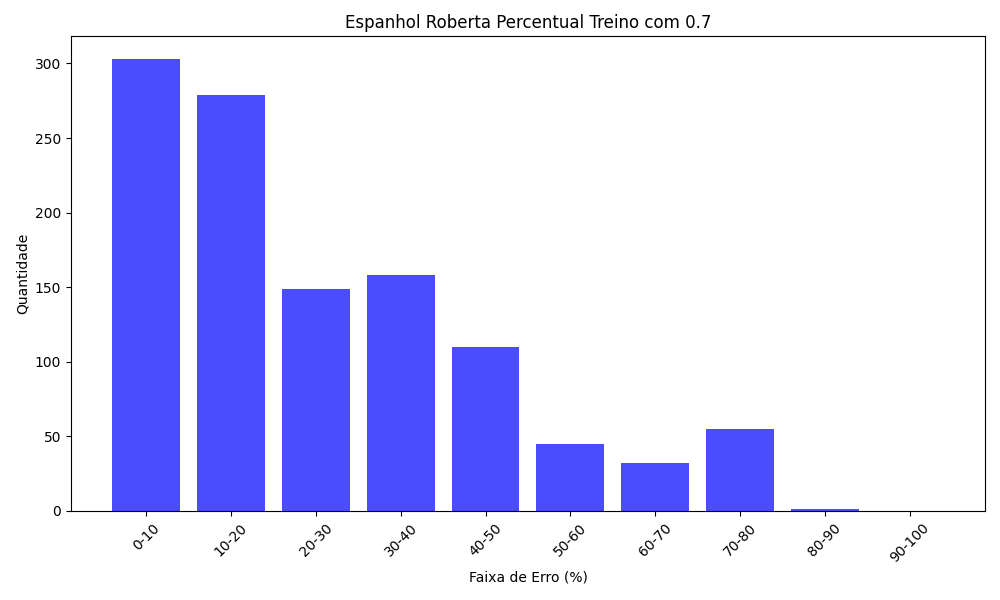
\includegraphics[width=\textwidth]{img/grafsEsp/Espanhol Roberta Percentual Treino com 0.7_quantidade.png}
\caption{Quantidade de respostas por faixas de erro percentual dos testes com 30\% do \textit{dataset} (Modelo Espanhol \textit{ROBERTA})}\label{figure:13}
\end{figure}

\begin{figure}[h!]
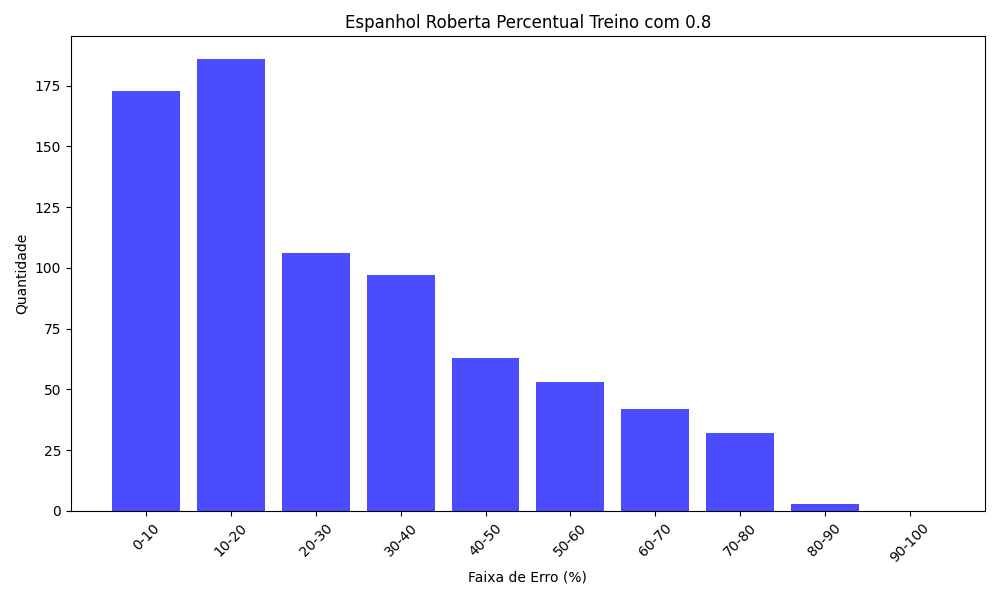
\includegraphics[width=\textwidth]{img/grafsEsp/Espanhol Roberta Percentual Treino com 0.8_quantidade.png}
\caption{Quantidade de respostas por faixas de erro percentual dos testes com 20\% do \textit{dataset} (Modelo Espanhol \textit{ROBERTA})}\label{figure:14}
\end{figure}

\begin{figure}[h!]
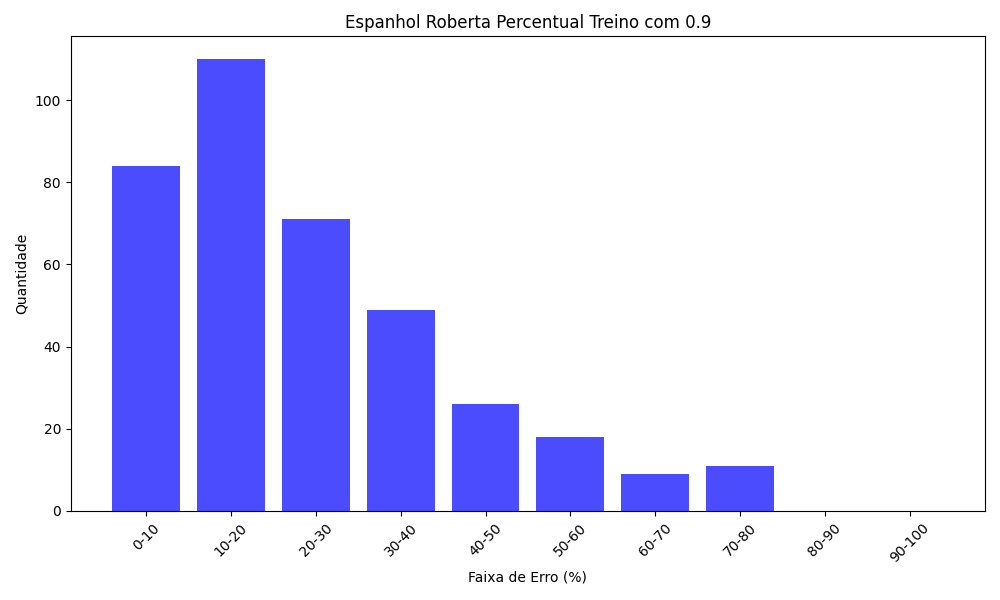
\includegraphics[width=\textwidth]{img/grafsEsp/Espanhol Roberta Percentual Treino com 0.9_quantidade.png}
\caption{Quantidade de respostas por faixas de erro percentual dos testes com 10\% do \textit{dataset} (Modelo Espanhol \textit{ROBERTA})}\label{figure:15}
\end{figure}

% \FloatBarrier

%------------ eng

\subsection{Resultados do treinamento com o \textit{dataset Mohler} (Inglês) usando o Modelo \textit{BERT Base}}

Os resultados do treinamento com o \textit{dataset Mohler} em inglês utilizando o modelo \textit{BERT Base} mostram que a acurácia média varia entre 78.15\% e 80.13\% conforme aumenta a quantidade de dados de treinamento. Observa-se que o EQM e o EMA diminuem ligeiramente à medida que mais dados são usados para treinamento, indicando uma melhoria na precisão do modelo. A melhor acurácia média foi alcançada com 70\% dos dados de treinamento.

\begin{table}[h!]
\centering
\resizebox{\columnwidth}{!}{%
\begin{tabular}{|p{0.25\textwidth}|p{0.1\textwidth}|p{0.1\textwidth}|p{0.4\textwidth}|p{0.1\textwidth}|p{0.1\textwidth}|p{0.1\textwidth}|}
    \hline
    \textbf{Percentual de dados para o treinamento} & \textbf{Qtd. Treino} & \textbf{Qtd. Teste} & \textbf{Pesos [Fator 1, Fator 2, Fator 3]} & \textbf{EQM} & \textbf{EMA} & \textbf{Acurácia média} \\
    \hline
    60\% & 2187 & 1459 & [0.4459, 0.1509, 0.1015] & 1.1724 & 0.8516 & 79.81\% \\
    \hline
    70\% & 2552 & 1094 & [0.4643, 0.1622, 0.1140] & 1.1672 & 0.8456 & 80.13\% \\
    \hline
    80\% & 2916 & 730 & [0.4469, 0.1705, 0.1459] & 1.1086 & 0.8242 & 78.79\% \\
    \hline
    90\% & 3281 & 365 & [0.4312, 0.1681, 0.1418] & 1.1034 & 0.8236 & 78.15\% \\
    \hline
\end{tabular}%
}
\caption{Resultados de Regressão para Diferentes Percentuais de Treino com o \textit{dataset Mohler} (Inglês) usando o Modelo \textit{BERT Base}}
\label{tab:resultados_regressao_ingles_base}
\end{table}

Nos gŕaficos das Figuras \ref{figure:16}, \ref{figure:17}, \ref{figure:18} e \ref{figure:19} é possível ver que a maiora das avaliações estão em uma faixa de acurácia acima de 80\%.

\begin{figure}[h!]
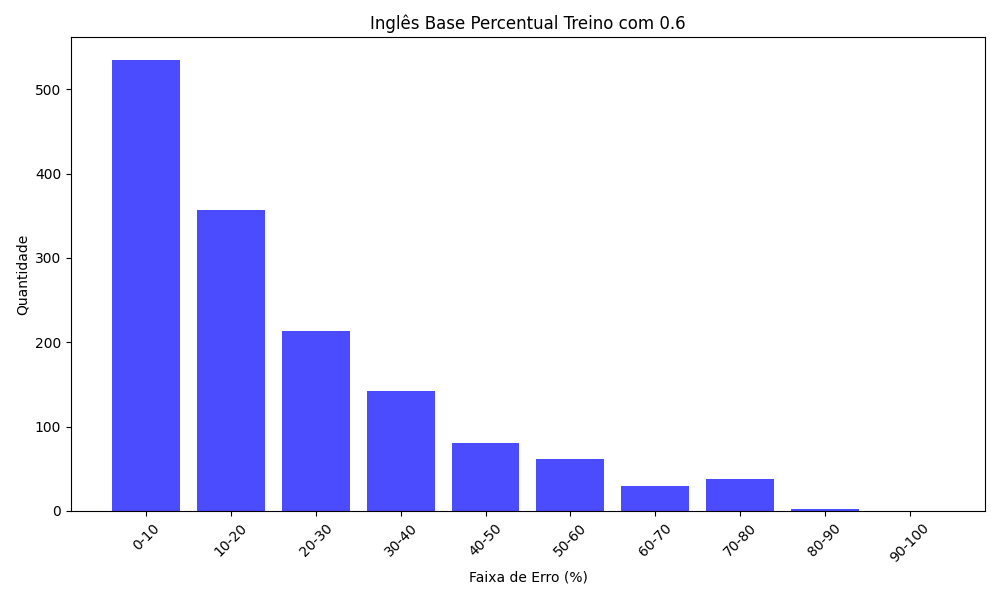
\includegraphics[width=\textwidth]{img/grafsEng/Inglês Base Percentual Treino com 0.6_quantidade.png}
\caption{Quantidade de respostas por faixas de erro percentual dos testes com 40\% do \textit{dataset Mohler} (Inglês) usando o Modelo \textit{BERT Base}}\label{figure:16}
\end{figure}

\begin{figure}[h!]
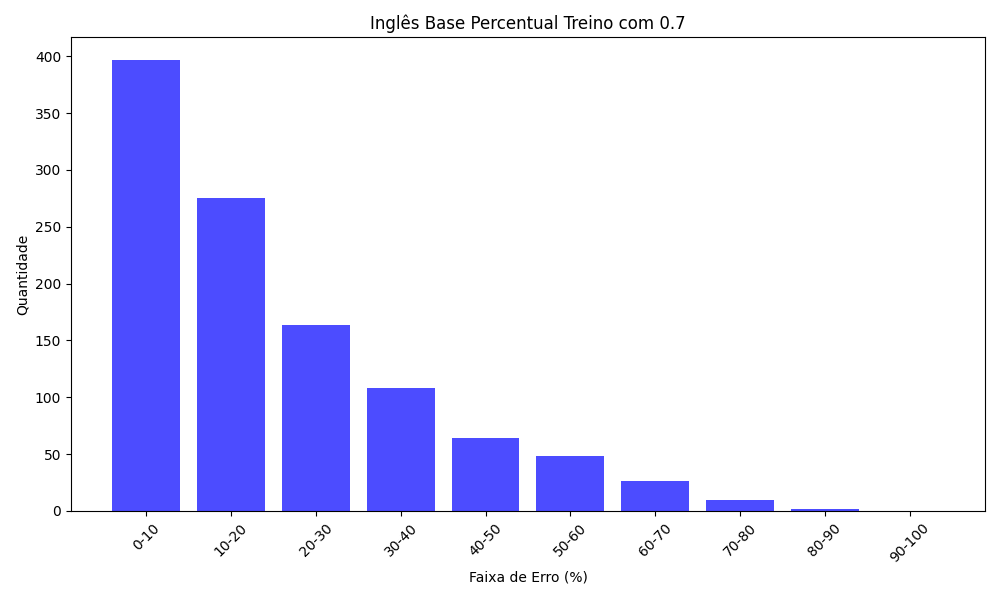
\includegraphics[width=\textwidth]{img/grafsEng/Inglês Base Percentual Treino com 0.7_quantidade.png}
\caption{Quantidade de respostas por faixas de erro percentual dos testes com 30\% do \textit{dataset Mohler} (Inglês) usando o Modelo \textit{BERT Base}}\label{figure:17}
\end{figure}

\begin{figure}[h!]
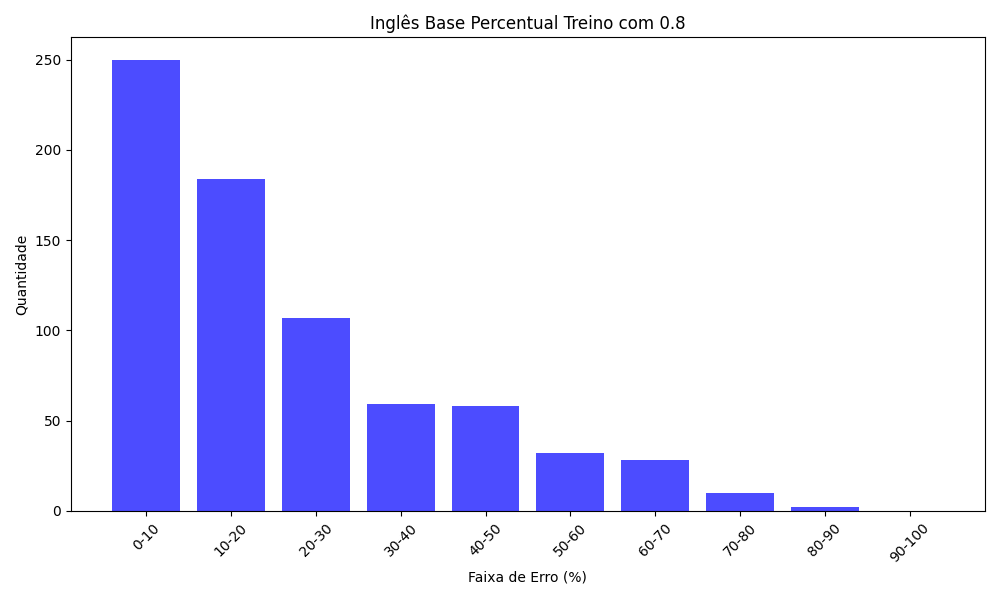
\includegraphics[width=\textwidth]{img/grafsEng/Inglês Base Percentual Treino com 0.8_quantidade.png}
\caption{Quantidade de respostas por faixas de erro percentual dos testes com 20\% do \textit{dataset Mohler} (Inglês) usando o Modelo \textit{BERT Base}}\label{figure:18}
\end{figure}

\begin{figure}[h!]
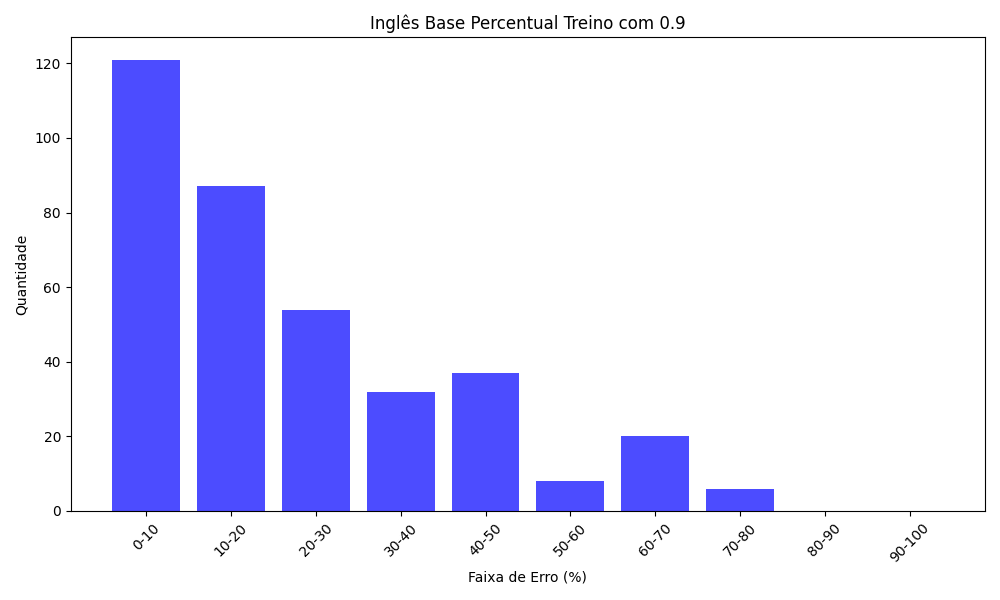
\includegraphics[width=\textwidth]{img/grafsEng/Inglês Base Percentual Treino com 0.9_quantidade.png}
\caption{Quantidade de respostas por faixas de erro percentual dos testes com 10\% do \textit{dataset Mohler} (Inglês) usando o Modelo \textit{BERT Base}}\label{figure:19}
\end{figure}

\FloatBarrier

%--------------------------------------------

\subsection{Resultados do treinamento com o \textit{dataset Mohler} (Inglês) usando o Modelo \textit{BERT Large}}

Os resultados do treinamento com o \textit{dataset Mohler} em inglês utilizando o modelo \textit{BERT Large} indicam uma melhoria geral em comparação ao modelo \textit{BERT Base}. A acurácia média varia de 79.72\% a 81.63\%, mostrando uma maior estabilidade e melhor desempenho com diferentes percentuais de dados de treinamento. Os valores de EQM e EMA também são consistentemente melhores, reforçando a eficácia do modelo \textit{BERT Large}.

\begin{table}[h!]
\centering
\resizebox{\columnwidth}{!}{%
\begin{tabular}{|p{0.25\textwidth}|p{0.1\textwidth}|p{0.1\textwidth}|p{0.4\textwidth}|p{0.1\textwidth}|p{0.1\textwidth}|p{0.1\textwidth}|}
    \hline
    \textbf{Percentual de dados para o treinamento} & \textbf{Qtd. Treino} & \textbf{Qtd. Teste} & \textbf{Pesos [Fator 1, Fator 2, Fator 3]} & \textbf{EQM} & \textbf{EMA} & \textbf{Acurácia} \\
    \hline
     60\% & 2187 & 1459 & [0.4473, 0.1388, 0.1930] & 1.1667 & 0.8519 & 81.19\% \\
    \hline
     70\% & 2552 & 1094 & [0.4698, 0.1487, 0.1814] & 1.1642 & 0.8451 & 81.63\% \\
    \hline
     80\% & 2916 & 730 & [0.4530, 0.1494, 0.1987] & 1.1072 & 0.8240 & 80.68\% \\
    \hline
     90\% & 3281 & 365 & [0.4388, 0.1487, 0.1727] & 1.1034 & 0.8237 & 79.72\% \\
    \hline
\end{tabular}%
}
\caption{Resultados de Regressão para Diferentes Percentuais de Treino com o \textit{dataset Mohler} (Inglês) usando o Modelo \textit{BERT Large}}
\label{tab:resultados_regressao_ingles_large}
\end{table}

Nos gŕaficos das Figuras \ref{figure:20}, \ref{figure:21}, \ref{figure:22} e \ref{figure:23} é possível ver que a maiora das avaliações se mantém na faixa de acurácia acima de 80\%, assim como no modelo \textit{Base}.


\begin{figure}[h!]
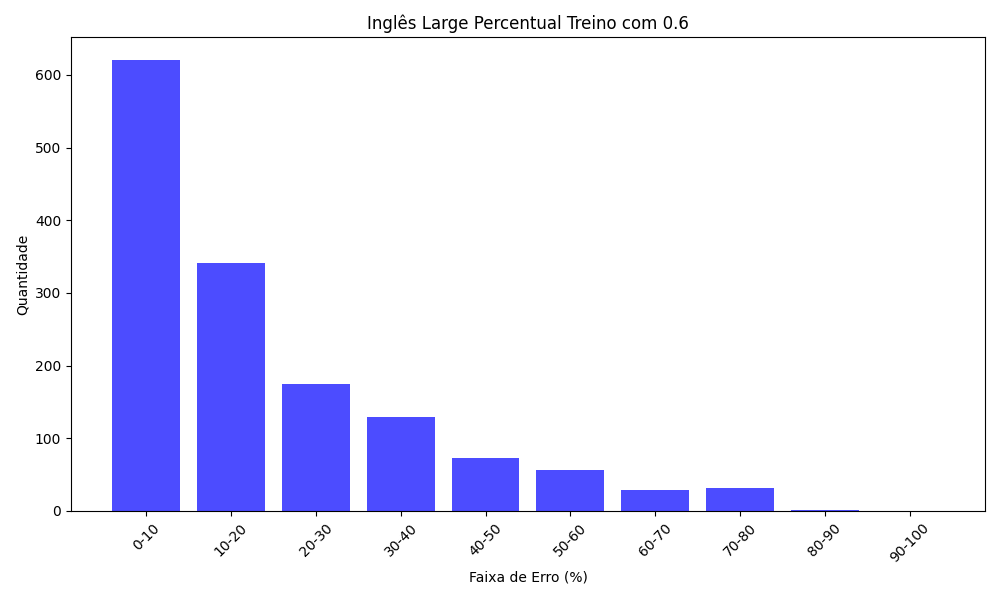
\includegraphics[width=\textwidth]{img/grafsEng/Inglês Large Percentual Treino com 0.6_quantidade.png}
\caption{Quantidade de respostas por faixas de erro percentual dos testes com 40\% do \textit{dataset Mohler} (Inglês) usando o Modelo \textit{BERT Large}}\label{figure:20}
\end{figure}

\begin{figure}[h!]
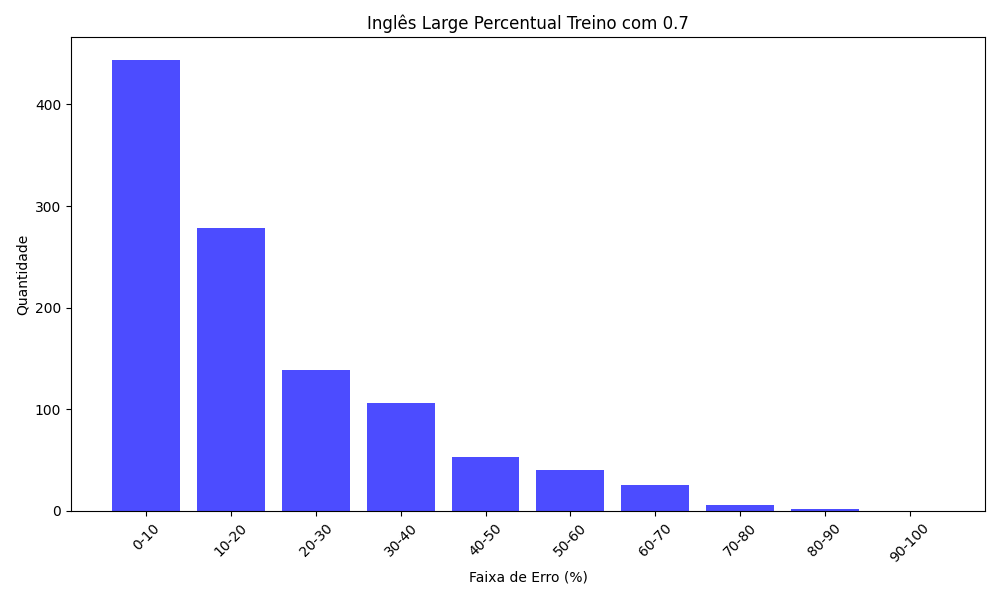
\includegraphics[width=\textwidth]{img/grafsEng/Inglês Large Percentual Treino com 0.7_quantidade.png}
\caption{Quantidade de respostas por faixas de erro percentual dos testes com 30\% do \textit{dataset Mohler} (Inglês) usando o Modelo \textit{BERT Large}}\label{figure:21}
\end{figure}

\begin{figure}[h!]
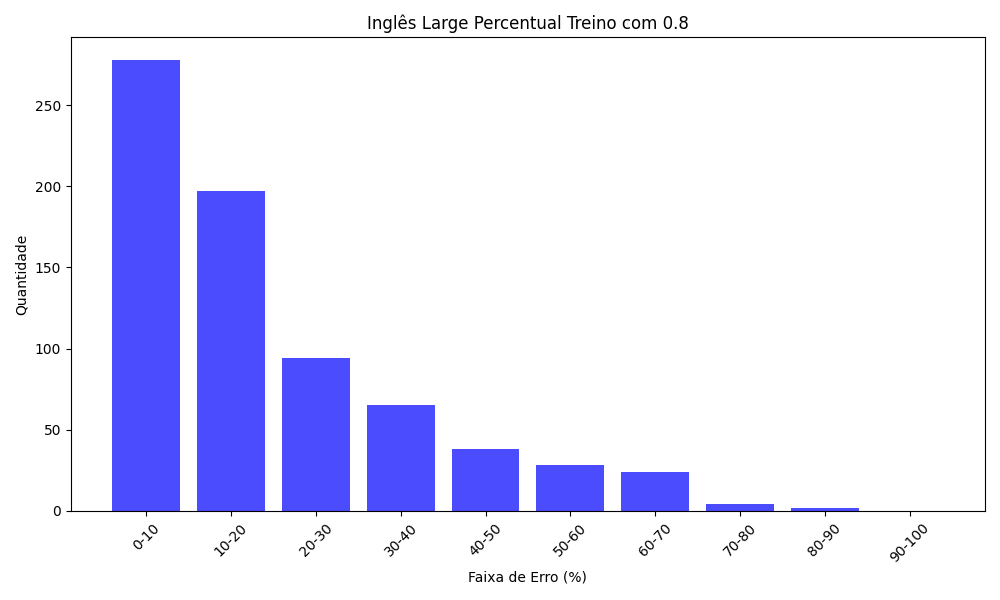
\includegraphics[width=\textwidth]{img/grafsEng/Inglês Large Percentual Treino com 0.8_quantidade.png}
\caption{Quantidade de respostas por faixas de erro percentual dos testes com 20\% do \textit{dataset Mohler} (Inglês) usando o Modelo \textit{BERT Large}}\label{figure:22}
\end{figure}

\begin{figure}[h!]
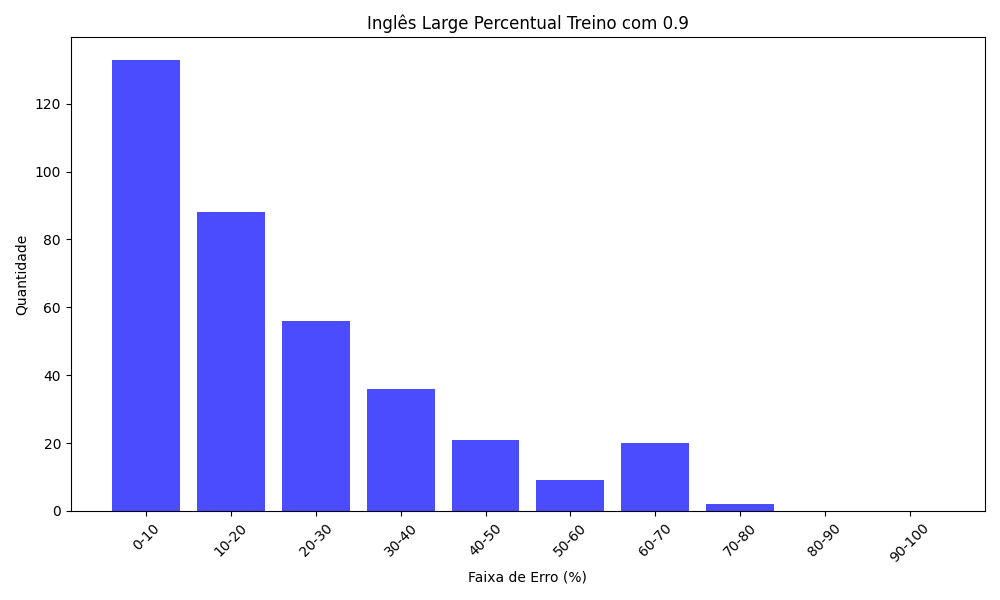
\includegraphics[width=\textwidth]{img/grafsEng/Inglês Large Percentual Treino com 0.9_quantidade.png}
\caption{Quantidade de respostas por faixas de erro percentual dos testes com 10\% do \textit{dataset Mohler} (Inglês) usando o Modelo \textit{BERT Large}}\label{figure:23}
\end{figure}

\FloatBarrier

\newpage

\subsection{Análise dos Resultados}

Os resultados obtidos indicam uma melhoria no desempenho do algoritmo à medida que mais dados de treinamento são utilizados. No entanto, mesmo com uma quantidade substancial de dados de treinamento, ainda há espaço para melhorias.

\subsubsection{Comparação entre os Conjuntos de Dados}

Ao comparar os resultados entre os conjuntos de dados em português, inglês e espanhol, observa-se que:

\begin{itemize}
    \item Para o conjunto de dados em português, o melhor resultado obtido foi de 63,43\%, enquanto para o conjunto de dados em espanhol, foi de 83.58\%. Já para o conjunto de dados em inglês, a taxa de erro geral foi de 81.63\%.
    \item As diferenças nos pesos otimizados entre os três conjuntos de dados podem indicar variações nas características mais importantes para cada idioma e também na quantidade de dados disponíveis no \textit{dataset} de cada um deles, o que pode ter afetado o resultado da regressão linear.
    \item Outras tendências ou discrepâncias grandes em valores de avaliações, podem ser exploradas para entender melhor como o algoritmo entendeu o fator para aquele texto e buscar compreender o sentido por trás das notas geradas nesses caso. Em tipos específicos de respostas, um fator pode estar pesando mais do que deveria. 
\end{itemize}

\section{Reprodutibilidade da experimentação}

Para que o experimento realizado no presente trabalho tenha transparência e integridade na sua condução, todos os códigos-fonte desenvolvidos ao longo do processo, juntamento com os dados de treinamento, testes e resultados obtidos estão todos disponibilizados públicamente no Github\footnote[1]{O repositório do Github pode ser acessado através do link: https://github.com/luca-moraes/relatorioParcialTCC}. Assim, qualque um pode executar os códigos para validação dos resultados apresentados neste trabalho ou, eventualmente, para comparação com outras possíveis abordagens propostas futuramente relacionadas a mesma temática deste trabalho.

\newpage